\documentclass[tikz,border=12pt]{standalone}
\usepackage[T1]{fontenc}
\usepackage{mathpazo}
\usepackage{amsmath,amssymb}
\usetikzlibrary{arrows.meta, positioning, calc, fit, patterns, decorations.pathreplacing}

\definecolor{stblue}{HTML}{7B97AD}
\definecolor{rwgold}{HTML}{B8995E}
\definecolor{sage}{HTML}{7A9A7E}
\definecolor{dkbrown}{HTML}{3D3530}
\definecolor{wmgray}{HTML}{7B7067}
\definecolor{cream}{HTML}{F9F6F0}
\definecolor{border}{HTML}{D4C9B8}
\definecolor{terracotta}{HTML}{C47A6A}
\definecolor{lavender}{HTML}{907EA0}

\begin{document}
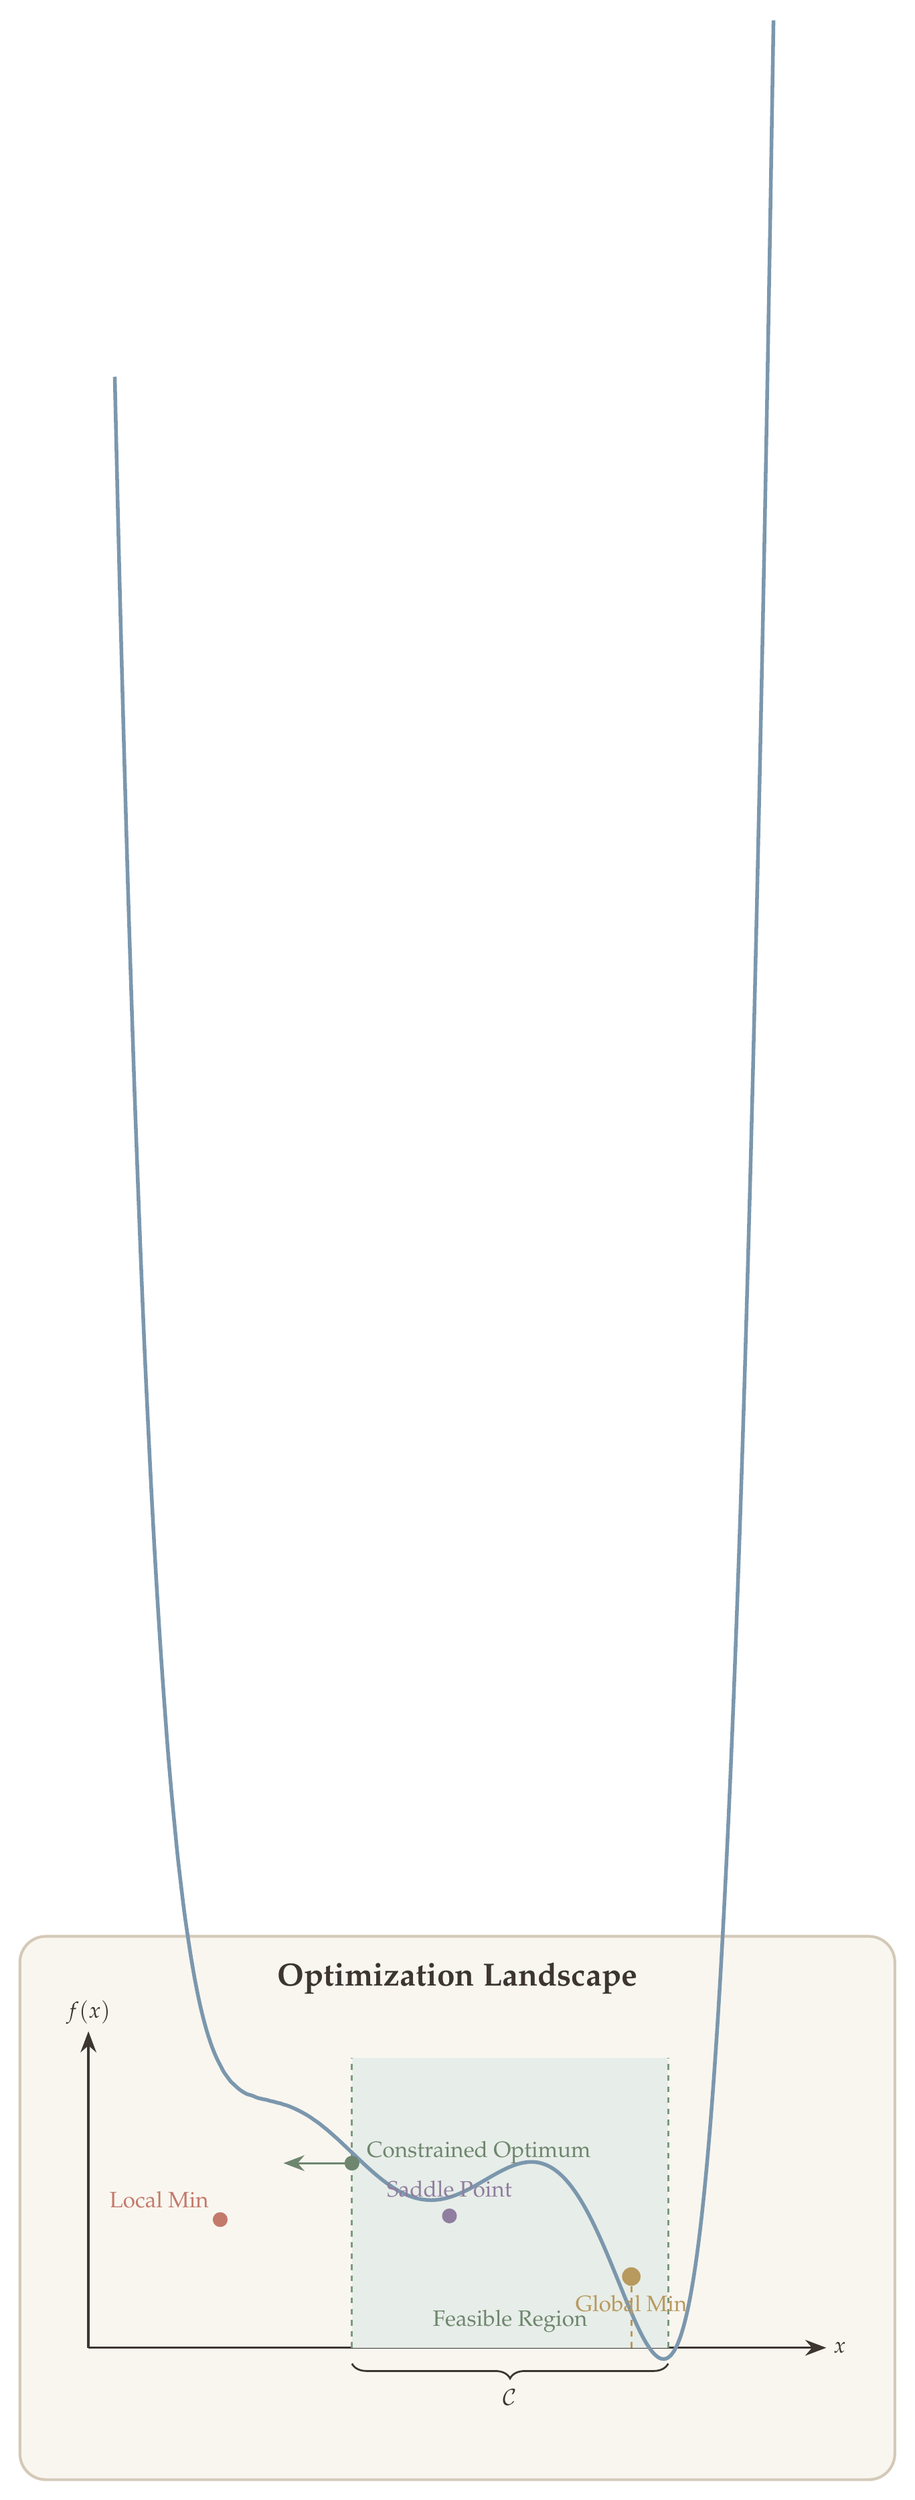
\begin{tikzpicture}[>={Stealth[length=4mm, width=3mm]}, line width=1.5pt]

% Background
\fill[cream, rounded corners=14pt] (-0.8,-2.5) rectangle (15.8,7.8);
\draw[border, line width=1.5pt, rounded corners=14pt] (-0.8,-2.5) rectangle (15.8,7.8);

% Title
\node[font=\LARGE\bfseries, text=dkbrown] at (7.5,7.0) {Optimization Landscape};

% Axes
\draw[->, dkbrown, line width=1.2pt] (0.5,0) -- (14.5,0) node[right, font=\large, text=dkbrown] {$x$};
\draw[->, dkbrown, line width=1.2pt] (0.5,0) -- (0.5,6) node[above, font=\large, text=dkbrown] {$f(x)$};

% Feasible region shading
\fill[sage!18] (5.5,0) rectangle (11.5,5.5);
\draw[sage, line width=1.2pt, dashed] (5.5,0) -- (5.5,5.5);
\draw[sage, line width=1.2pt, dashed] (11.5,0) -- (11.5,5.5);
\node[font=\large, text=sage!80!dkbrown] at (8.5,0.5) {Feasible Region};

% Function curve
\draw[stblue, line width=2pt, smooth, samples=200, domain=1:13.5]
  plot (\x, {0.0018*(\x-3)^2*(\x-7)^2*(\x-11)^2 - 0.04*(\x-7)^3 + 2.8});

% Local minimum (around x=3)
\fill[terracotta] (3,2.43) circle (4pt);
\node[font=\large, text=terracotta, above left=3pt] at (3,2.43) {Local Min};

% Saddle point (around x=7)
\fill[lavender] (7.35,2.5) circle (4pt);
\node[font=\large, text=lavender, above=6pt] at (7.35,2.5) {Saddle Point};

% Global minimum (around x=11)
\fill[rwgold] (10.8,1.35) circle (5pt);
\node[font=\large, text=rwgold, below=6pt] at (10.8,1.35) {Global Min};
\draw[rwgold, line width=1pt, dashed] (10.8,0) -- (10.8,1.35);

% Constrained optimum on feasible region boundary
\fill[sage!80!dkbrown] (5.5,3.5) circle (4pt);
\draw[sage!80!dkbrown, line width=1pt, ->] (5.5,3.5) -- (4.2,3.5);
\node[font=\large, text=sage!80!dkbrown, right=4pt] at (5.5,3.7) {Constrained Optimum};

% Annotations with braces
\draw[decorate, decoration={brace, amplitude=8pt, mirror}, dkbrown, line width=1pt]
  (5.5,-0.3) -- (11.5,-0.3) node[midway, below=10pt, font=\large, text=dkbrown] {$\mathcal{C}$};

\end{tikzpicture}
\end{document}
